\documentclass[12pt]{report}
\usepackage[utf8]{inputenc}
\usepackage{graphicx}
  \graphicspath{ {figures/} {chapters/pileup/figures/} {chapters/pileup2/figures/} }
\usepackage{subcaption}
\usepackage{amsmath}
\usepackage{amsfonts}
\usepackage{hyperref}
\hypersetup{
    colorlinks,
    citecolor=black,
    filecolor=black,
    linkcolor=black,
    urlcolor=black
}

\newcommand{\myname}{PUMiNet}

\title{
  {Standard Model of Particle Physics\\ and Machine Learning}\\
  {\large Oklahoma State Univeristy}\\
  {\hfill}\\
  {
\includegraphics[width=0.2\textwidth]{Oklahoma_State_University_seal.png}}
}
\author{Luke Martin Vaughan}
\date{Expected Completion: Spring 2026}

\begin{document}

\maketitle

\tableofcontents

%\chapter*{Abstract}
%Abstract goes here.


%\chapter*{Dedication}
%Dedication goes here.


%\chapter*{Declaration}
%Declaration goes here.


%\chapter*{Acknowledgements}
%Acknowledgements goes here.


\chapter{Introduction}
\section{The Standard Model of Particle Physics}

The standard model of particle physics explains the fundamental forces of nature.

\begin{figure}[h]
  \centering
  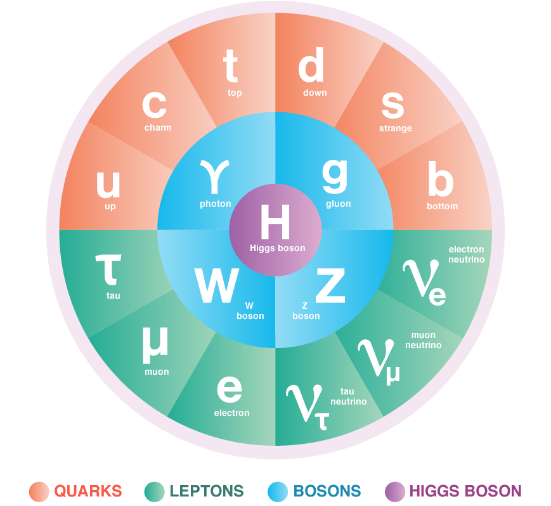
\includegraphics[width=0.5\textwidth]{SM.png}
\end{figure}


\appendix
\chapter{Pileup Studies}
\section{Introduction}\hfill

% The Large Hadron Collider~\cite{LHC}, LHC, is the largest and highest energy particle collider ever constructed by humankind. Using superconducting magnets, protons are accelerated around a 27km ring and collide in designated interaction points at a center of mass energy of 14TeV. The proton-proton interactions produce heavy particles which decay into a higher multiplicity of lighter particles. This decay chain results in a cascading effect which creates a shower of particles observed by the detector. If particles originate from a common heavy ancestor, they often form collimated streams of lighter particles in a tight cone, which are referred to as jets.

High Energy Particle physicists study proton-proton collisions at the Large Hadron Collider (LHC)~\cite{LHC} to better understand phenomena of the universe related to the fundamental forces of nature. These proton-proton collisions produce particles that are irreducible quanta of energy.
%described by the Standard Model of Particle Physics. 
Due to the subatomic size of protons, the mean number of interactions per bunch crossing in billions, $\left\langle \mu \right\rangle$, is very small. Only one of these collisions interacts via a strong head-on collision that produces deep inelastic scattering called \emph{hard scatter} or \emph{signal}, while other weaker interactions are called \emph{pileup} or \emph{background}. 
%In addition to hard scatter, there exists many other soft collisions arising from weaker interactions which are called \emph{pileup}. 
Each of these collisions, in turn, produces heavy particles which decay into lighter particles in a cascading effect. Streams of such decayed particles are called \emph{jets}, which can be clustered to form a tightly knit cone containing charged particles, called \emph{tracks}. All these collisions are recorded as \emph{events}, usually at a rate of every 25 nanoseconds, containing a variable number of jets and a variable number of tracks in each jet. It is important to note that jets originating from hard scatter processes share underlying physics and thus can be correlated with other jets in the hard scatter process. Such a correlation is not feasible for pileup jets due to their stochastic nature, as given in Figure~\ref{fig:PileupJets}.

%The Large Hadron Collider~\cite{LHC}, LHC, is the largest and highest energy particle collider ever constructed by humankind. Using superconducting magnets, protons are accelerated around a 27km ring and collide in designated interaction points at a center of mass energy of 14TeV. This decay chain results in a cascading effect which creates a shower of particles observed by the detector.
%The proton-proton interactions that happen in colliders like Large Hadron Collider~\cite{LHC} produce heavy particles which decay into a higher multiplicity of lighter particles in a cascading effect. 
%\textcolor{red}{We need to simplify these two sentences.} Streams of such lighter particles originating from a common ancestor are called \emph{jets}, they often form collimated streams of lighter particles in a tight cone, which are referred to as jets.

%General purpose detectors at the LHC consist of two main components: a tracker and a calorimeter. The tracker uses silicon dots and strips to measure the position and momentum of each particle that passes through it. Particles that are reconstructed using the tracker are referred to as tracks. The calorimeter uses dense material, such as lead, to absorb and record the energy of particles. A stream of collimated particles that deposits energy into the calorimeter is reconstructed as a jet.

%Due to the very small interaction cross-section of proton-proton collisions, bunches of 100 billion protons are collided at the same time to increase the rate of interaction. On average, there will be zero or one collisions that interact "head on" producing deep inelastic scattering. This type of interaction is called the Hard Scatter, HS, process. However, in the current LHC configuration, there exists, on average, an additional 60 other interactions from various protons in the bunch crossing that are physically piled up on top of the hard scatter interaction. These additional interactions are referred to as Pileup, PU, processes.

\begin{figure}[h]
\centering
\begin{subfigure}{.45\textwidth}
  \centering
  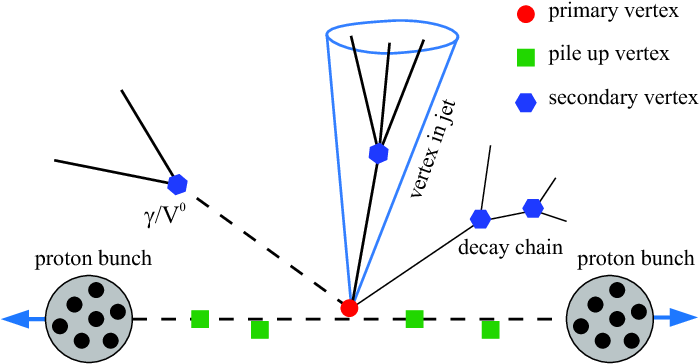
\includegraphics[width=1\linewidth]{Vertexing.png}
  \caption{}
  \label{fig:sub1}
\end{subfigure}%
\begin{subfigure}{.45\textwidth}
  \centering
  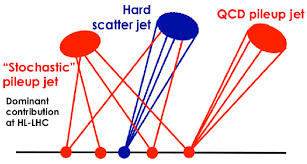
\includegraphics[width=1\linewidth]{StochasticPileup}
  \caption{}
  \label{fig:sub2}
\end{subfigure}
  \caption{As the proton bunches cross and interact, there typically exists one hard scatter interaction originating from the primary vertex while the other interactions originate from pileup vertices. The jets that originated from the HS vertex form a correlated set, while the jets from PU are stochastic in nature and do not have correlations. Remake this graphic and combine!}
\label{fig:PileupJets}
\end{figure}

Pileup interactions are considered as contamination because of their massive quantities compared to signal processes. It is important to identify and mitigate pileup from collision events to increase sensitivity of signal processes and assist physicists to discover new particles. Many data science and AI approaches have been introduced in recent years to mitigate pileup in variety of ways. All related work goes here.

Although there is growing interest in this domain, existing methods  assume (i) only low pileup events, and (ii) pileup identification as a binary classification problem Find citations. As LHC prepares to upgrade to the High-Luminosity (HL)LHC~\cite{HLLHC}, with $\left\langle \mu \right\rangle = 200$, it brings several billion collisions with exponentially higher number of pileup processes. Explain $\mu$ values used in existing works and why it will be a problem for $\mu = 200$. In low pileup conditions, the data is sparse such that jets can be easily binary classified as hard scatter or pileup jets. There could be a few pileup tracks entering a hard scatter jet, which can be corrected using Charged Hadron Subtraction~\cite{CHS}, but the overall mass and energy of the hard scatter jet are seemingly unaffected. This becomes challenging with the upcoming upgrades to LHC which introduces several noisy pileup tracks into hard scatter jets and eventually altering core properties of hard scatter jets.

%\In low pileup conditions, pileup is sparse enough such that jets tend to be binary classified as hard scatter or pileup jets as shown in figure \ref{fig:PileupJets}. There could exist a few tracks entering a hard scatter jet, which can be corrected using Charged Hadron Subtraction~\cite{CHS}, but the overall mass and energy of the hard scatter jet are seemingly unaffected. However if pileup increases, there exists a critical point in $\left\langle \mu \right\rangle$ where there is such a large pileup background that the mass and energy of hard scatter jets are significantly affected.
%This critical point becomes more daunting as the LHC prepares to upgrade to the High-Luminosity (HL)LHC~\cite{HLLHC}. The HL-LHC will bring in much more data for hard scatter collisions at the cost of many more pileup collisions.

The existing algorithms developed for pileup mitigation using binary classification at low pileup conditions for the LHC will start to struggle as pileup is increased for the HL-LHC. Therefore at high pileup conditions, future algorithms must consider pileup as continuous regression problem to determine by what fraction the \emph{hard scatter} jet's mass and energy has been affected by \emph{pileup}. In this paper we propose a model that attemphts to solve the problem of pileup by directly predicting energy and mass fractions of each jet using transformer encoders using self-attention and cross-attention to learn enriched representations of jets using all possible correlations between jets and tracks within the context of an event.

% Explain why it is necessary to identify pileup jets for physics processes. Processes that lead to new physics, considered as signal, occur through \emph{hard scatter} interactions. All other interactions are considered \emp{pileup} and are a source of background which contaminates the signal. Therefore, the identification and suppression of the \emp{pileup} background is crucial to increase the sensitivity to signal of the \emp{hard scatter} processes. Pileup mitigation helps physicists to probe new physics and discover new particles by reducing the pileup background.

In this work, we present the following contributions.
\begin{enumerate}
    \item We propose a first-of-its-kind pileup prediction modeled as a regression problem.
    \item We propose cross-attention based neural network architecture that utilizes jets and tracks information for pileup fraction detection.
    \item We show with extensive analysis that the proposed method outperforms the baseline approaches.
    \item We also show that the predictions from the proposed approach also assist with physics processes.
\end{enumerate}

%An event is defined as data recorded from a single bunch crossing which occur every 25 nanoseconds. Each event contains variable length set of jets. Each jet contains a variable length set of tracks. The hard scatter jets that originate from the same underlying physics process will be correlated with each other. On the other hand, pileup jets are formed due to stochastic nature and are not correlated to other jets in the event. Attention neural networks are capable of learning correlations between jets and allow for a context window of an entire event.

% \begin{figure}[h]
%   \centering
%   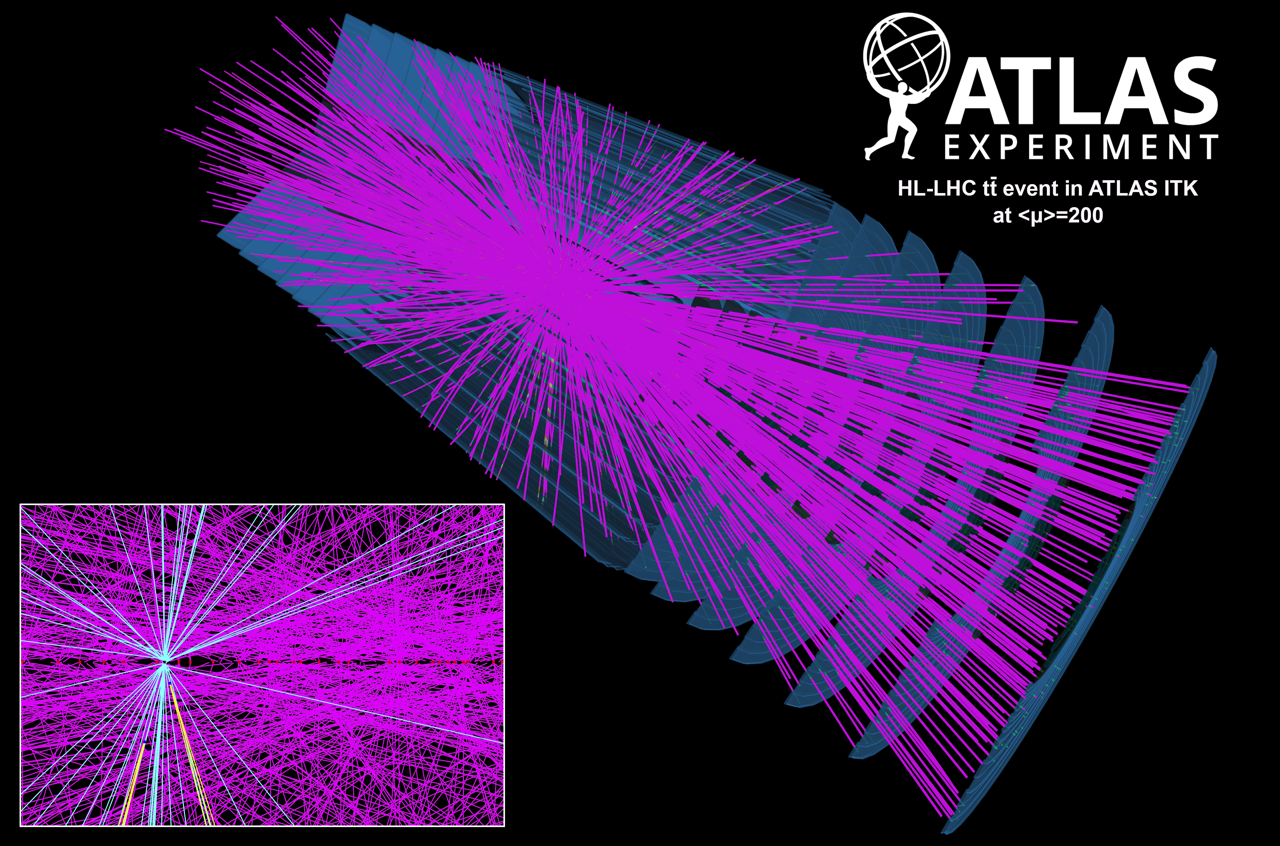
\includegraphics[width=0.75\linewidth]{HL-LHC-tt}
%   \label{fig:vertexing}
%   \caption{In the HL-LHC configuration, the Hard Scatter process (light blue) begins to be dominated by PileUp (purple). Note: https://atlas.cern/updates/news/scientific-potential-high-luminosity-lhc}
% \end{figure}



%In order to increase the amount of data collected, the LHC has plans to plans to increase the mean number of collisions, $\left<\mu\right>$, for what is called the High-Luminosity (HL)LHC~\cite{HLLHC}. The HL-LHC will increase the mean number of interactions up to $\left<\mu\right>=200$ to collect more data and increase statistics. This change in configuration of the LHC will bring much more pileup begins to dramatically blur the concept of a HS and PU jet. What was a binary classification task at low pileup conditions becomes a continuous regression task at high pileup conditions. This is due to the fact that there are so many pileup particles crammed into the $4\pi$ solid angle coverage of the detector, that nearly all hard scatter jets have a significant contribution to their mass and energy from pileup. 

%This motivates that jets should not be considered as binary HS or PU, but instead jets should have a continuous energy and mass corrections that are be applied to correct for pileup effects. In this paper, we propose an improvement to pileup mitigation at the HL-LHC using Multi-Head Attention and Transformer Encoder stacks~\cite{Attention} to perform a continuous regression task on jets in the context of an entire event. \\


\section{Related Work}\hfill

Machine learning approaches for High Energy Physics problems are gaining traction from multiple perspectives with advancements in neural networks~\cite{he2023high,Barman_2024,Larkoski_2020}. Although there are several sub-problems in High Energy Physics, such as jet flavor tagging~\cite{qu2022particle`}, top tagging, generative event modeling~\cite{kansal2021particle}, unfolding, anomaly detection, and calibration that have been explored with machine learning, methods to analyze \emph{PileUp} have been mostly overlooked in the existing work. One of such interesting problems is mitigating pile-up particles and correcting jet mass and energy for events that occur at the Large-Hadron Collider~\cite{komiske2017pileup}. \\ 

Existing pileup mitigation techniques for the ATLAS and CMS experiments have focused on solving the binary classification problem for either jets or tracks. ATLAS uses algorithms to classify jets using classifiers such as kNN algorithms~\cite{ATLAS-CONF-2014-018} which rely on constructing high level variables on a per jet basis. CMS uses an algorithm to classify tracks using a statistical $\chi^2$ approach through the PUPPI~\cite{Bertolini_2014} algorithm classifies pileup at the particle level. However, these methods fail to incorporate correlations between jets at the Event level for Event-Wide context. Correlations exists between jet originating from Hard Scatter processes.  \\

Graph Neural Networks have also been studied for for pileup mitigation, however, it is non-trivial how to form a graph in the context of an event. Its unfeasible to connect all particles in an event due to computation limitations, and connecting all tracks within a jet can confuse the model unless edge weights are assigned properly for HS and PU particles. Dynamic edge convolutions have been studied, but this can lead to long training times due to calculating kNN in latent space. Attention, on the other hand, gives a highly parallelizable algorithm to automatically determine weights between objects and update node representations accordingly.

\section{Jet Corrections in High Pileup Conditions}\hfill

As $\left<\mu\right>$ increases from 60 to 200 for the HL-LHC upgrade, the pileup contamination of hard scatter jets will begin to dominate. As PU contamination degrades the quality of HS jets, the task shifts from a binary classification at low pileup conditions to a continuous regression at high pileup conditions. Instead of the traditional binary labels as HS or PU, we introduce a continuous labels for Energy and Mass Fraction, Efrac and Mfrac, which represents the fraction of the jets energy and mass originating from pileup.

To construct these continuous labels, we sum over the Lorentz Four-Vector of the tracks, $\vec{T_i} = (E,p_x,p_y,p_z)_i = (E,\vec{p})_i = (T_0, T_1, T_2, T_3)_i$, which are truth-associated to each jet, $\vec{J}$:

\begin{equation}
    \vec{J}_{HS} = \sum_{i \in \text{HS}} \vec{T}_i \phantom{............} \vec{J}_{PU} = \sum_{i \in \text{PU}} \vec{T}_i \\
    %\vec{J}_{Total} = \vec{J}_{HS} + \vec{J}_{PU} 
\end{equation}

Now that we have the four vector HS and PU contributions of each jet, we can directly evaluate the Energy and Mass fractions on a per jet basis. The total Lorentz Four-Vector is simply the sum of the HS and PU contributions, $\vec{J}_{Total} = \vec{J}_{HS} + \vec{J}_{PU}$. Note that Energy is the first component of the jets Four-Vector, $J_0=E$, and mass is found using the relativistic energy relations in natural units, $m^2=E^2-|\vec{p}|^2$. These expressions can be used to derive the labels used for regression.

\begin{equation}   
    Efrac = \frac{E_{HS}}{E_{Total}} \phantom{............} Mfrac = \frac{m_{HS}}{m_{Total}}
\end{equation}

\begin{figure}[h]
\centering
\begin{subfigure}{.35\textwidth}
  \centering
  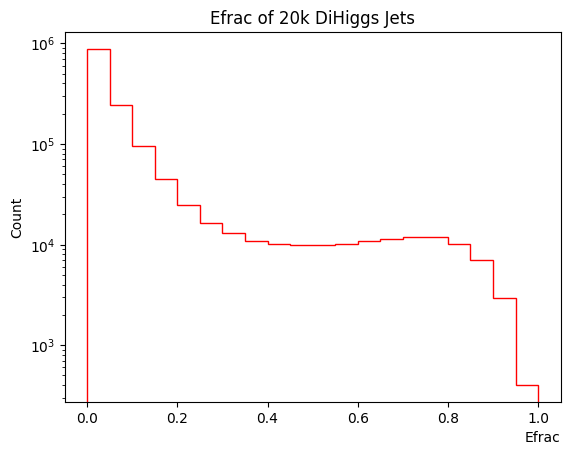
\includegraphics[width=1\linewidth]{Efrac}
  \caption{}
  \label{fig:sub1}
\end{subfigure}%
\begin{subfigure}{.35\textwidth}
  \centering
  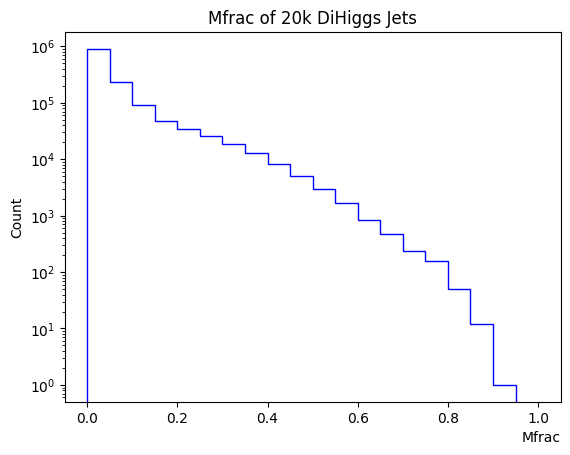
\includegraphics[width=1\linewidth]{Mfrac}
  \caption{}
  \label{fig:sub2}
\end{subfigure}
\caption{The truth energy and mass fractions used for the continuous regression task at $\left< \mu \right> = 60$.}
\label{fig:test}
\end{figure}

These continuous labels allow for corrections to be applied directly to the jet mass and energy. Of course a proper calibration will need to be applied when evaluated on data.


\section{Simulated Dataset}\hfill

A sample of 100k $pp \rightarrow HH$ events were generated using MADGRAPH\_AMC@NLO~\cite{Alwall_2014} and showered through $H \rightarrow b\bar{b}$ channel using Pythia8~\cite{bierlich2022comprehensiveguidephysicsusage}. As each hard scatter process is showered in Pythia, pileup processes are overlaid using SoftQCD:inelastic generated with the A14 central tune with NNPDF2.3LO~\cite{bierlich2022comprehensiveguidephysicsusage}. The average number of pileup processes are controlled by parameter $\left<\mu\right>$ which follows a poisson distribution. Each pileup vertex undergoes gaussian smearing where the width in the x and y directions, representing the beam width, are 0.3mm and the spread in the z direction is 50mm. Stable final state particles are then passed to FastJet~\cite{Cacciari_2012} to be cluster into jets using $anti-k_t$ algorithm~\cite{Cacciari_2008} with R=0.4 and minimum $p_T$ of 25 GeV. \\

\begin{figure}[h]
\centering
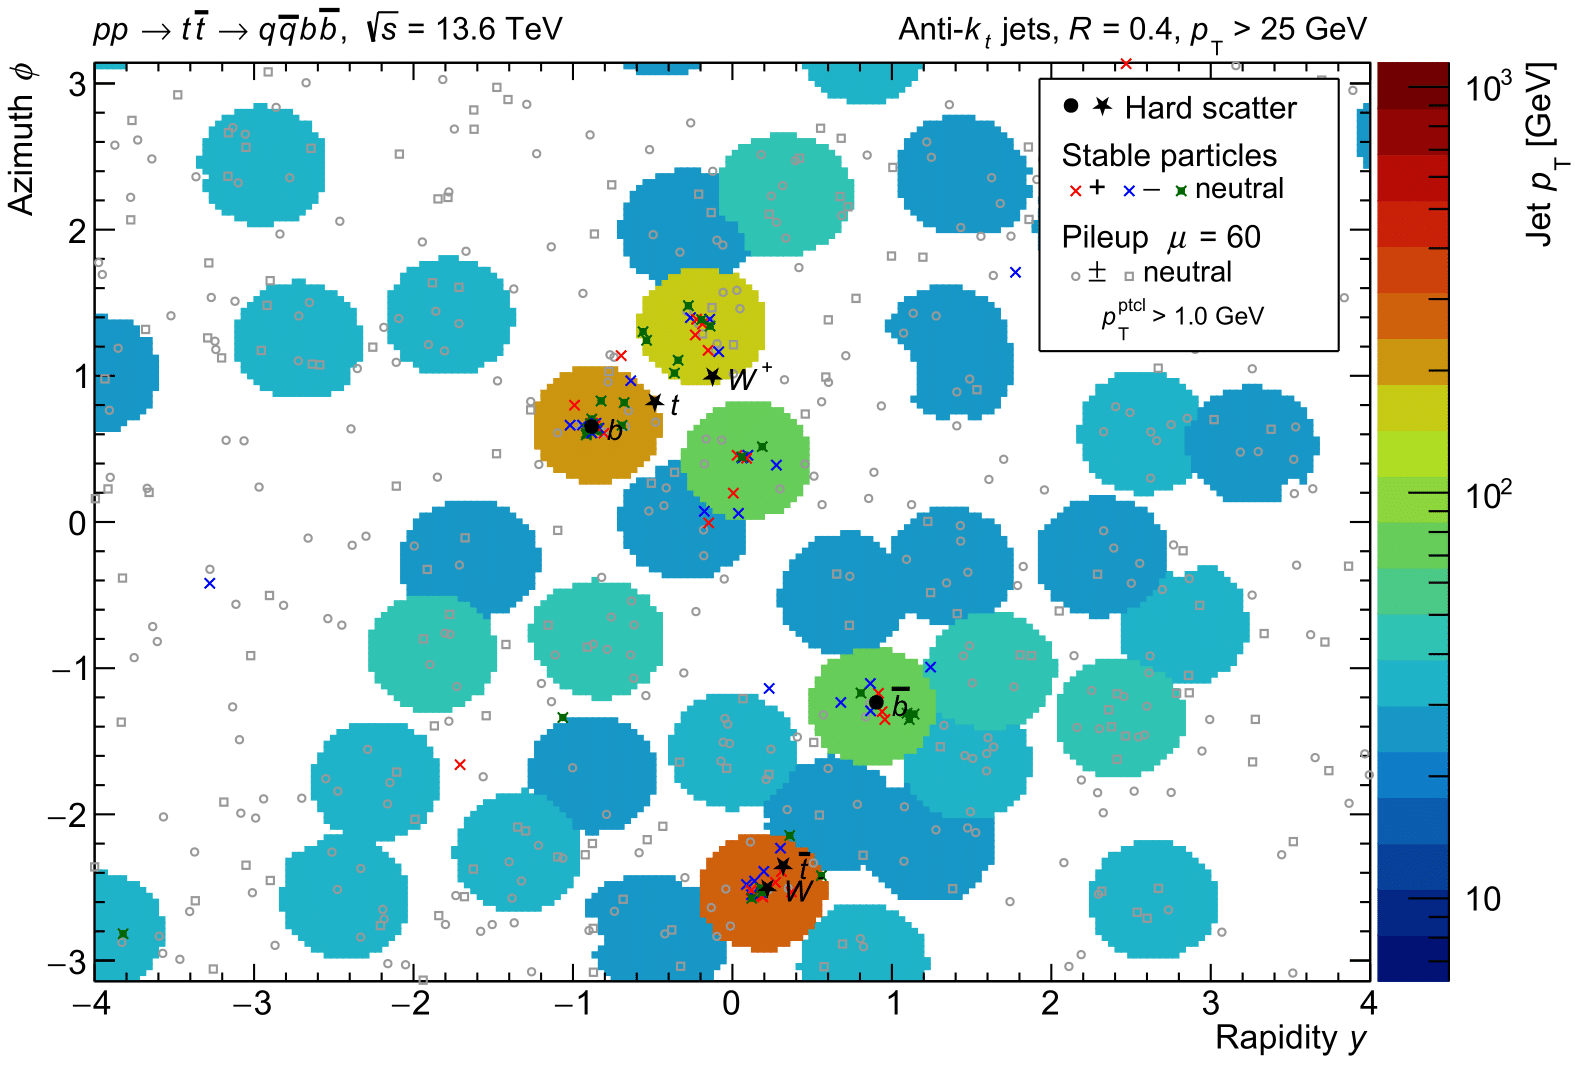
\includegraphics[width=0.65\textwidth]{Event}
\caption{An example of a simulated event of $pp \rightarrow t\bar{t}$ decaying hadronically at $\left< \mu \right> =60$.}
\end{figure}

To incorporate detector limitations, neutral particles and particles below 400 MeV were cut from the training dataset. After cuts, the dataset contains 500k jets and 10M particles. However, it is important to note that the jets studied in this paper are not calorimeter jets, but instead more idealistic track-jets. The results from this study offer the best-case scenario when tracks can be perfectly assigned the correct vertex, and the performance would be expected to degrade slightly in realistic detector conditions.

\section{Improving JVT using Attention}\hfill

The JVT model used by ATLAS is used to classify jets as HS or PU. However, at high pileup conditions JVT algorithm will need to be improved. Here we benchmark the JVT kNN algorithm~\cite{ATLAS-CONF-2014-018} against AttnJVT.
\subsection{Jet Features}\hfill

Each jet has 6 features which includes the kinematic 4-vector of each jet, $p_T, \eta, \phi, m$ as well as track dependent features $corrJVF, Rp_T$ which were first proposed by ATLAS~\cite{ATLAS-CONF-2014-018}. First, corrJVF can be understood as the fraction of the jet's momentum coming from hard scatter particles originating from the primary vertex with respect to the total momentum coming from all other vertices. However, it has been shown that this variable has a dependence on $\left<\mu\right>$, so to correct for this behavior the contribution from pileup vertices are normalized by the number of pileup particles in the event and a free parameter, k. This parameter has been shown to best remove dependence on $\left<\mu\right>$ at k=0.01~\cite{ATLAS-CONF-2014-018}.
\begin{equation}
    corrJVF = \frac{\sum\limits_k p_T^{trk_k}(PV_0)}{\sum\limits_l p_T^{trk_l}(PV_0)+\frac{\sum\limits_{n\geq1}\sum\limits_l p_T^{trk_l}(PV_n)}{(k \cdot n^{PU}_{trk})}}
\end{equation}

%\begin{figure}[h!]
%\centering
%\begin{subfigure}{.45\textwidth}
%  \centering
%  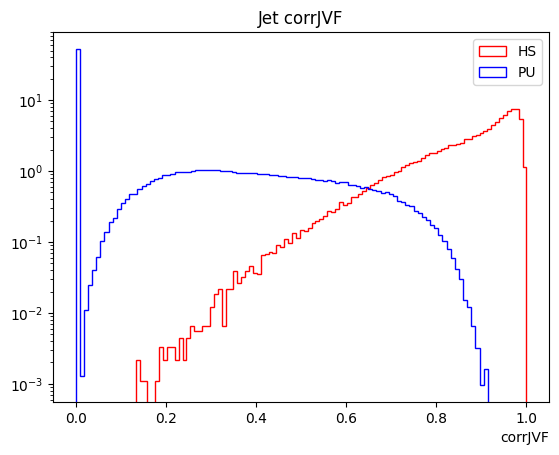
\includegraphics[width=0.9\linewidth]{corrJVF}
%  \caption{}
%  \label{fig:sub1}
%\end{subfigure}
%\begin{subfigure}{.45\textwidth}
%  \centering
%  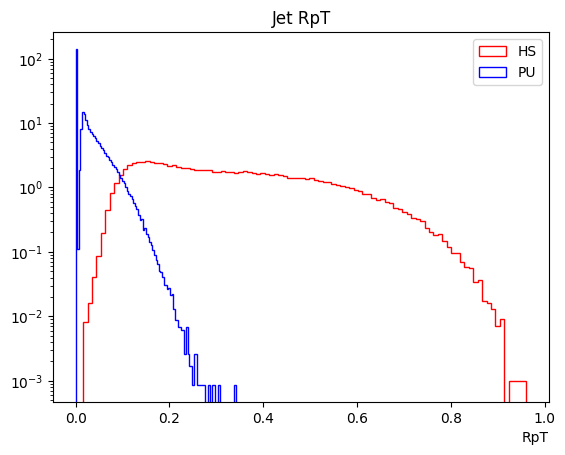
\includegraphics[width=0.9\linewidth]{RpT}
%  \caption{}
% \label{fig:sub2}
%end{subfigure}
%\caption{Figure (a) The distribution of corrJVF for Hard Scatter jets and PileUp jets.. Figure (b) The %istribution of $R_{pT}$ for Hard Scatter jets and PileUp jets.}
%label{fig:test}
%\end{figure}

Second, $R_{pT}$ can be understood as the fraction of the jet's momentum originating from hard scatter primary vertex.
\begin{equation}
    R_{pT} = \frac{\sum_kp_T^{trk_k}(PV_0)}{p_T^{jet}}
\end{equation}

These features have unique distributions for HS and PU jets. HS jets tend to have higher corrJVF and RpT than pileup jets as shown in figure [*]. \\

\begin{figure}[h!]
\centering
\begin{subfigure}{.25\textwidth}
  \centering
  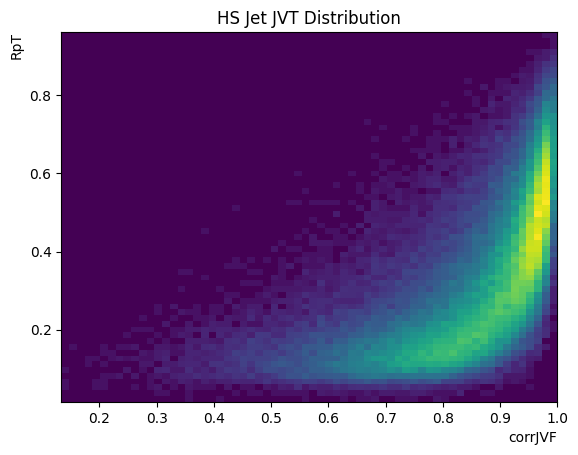
\includegraphics[width=0.9\linewidth]{HS}
  \caption{}
  \label{fig:sub1}
\end{subfigure}%
\begin{subfigure}{.25\textwidth}
  \centering
  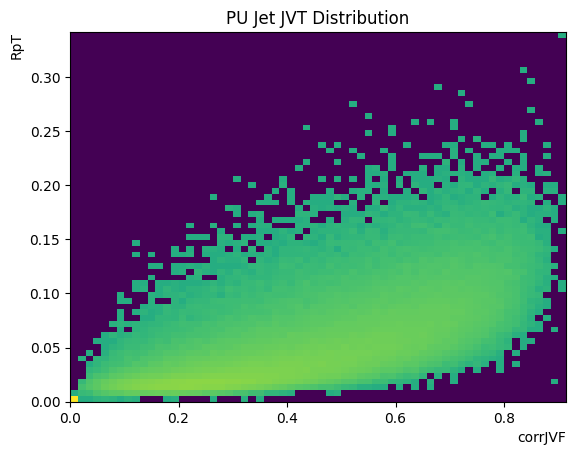
\includegraphics[width=0.9\linewidth]{PU}
  \caption{}
  \label{fig:sub2}
\end{subfigure}
\caption{Distribution of jets in the $R_{pT}$-corrJVF plane for (a) HS and (b) PU jets.}
\label{fig:test}
\end{figure}

\subsection{Jet Labels}\hfill

To fairly benchmark JVT and AttnJVT, a binary label was constructed by cutting on the squared sum of the constituent particle's $p_T$.

\begin{equation}
    PU_{fr} = \frac{\sum\limits_{PU} p_T^{2}}{\sum\limits_{HS} p_T^{2} + \sum\limits_{PU} p_T^{2}}
\end{equation}

An arbitrary cut is imposed on this distribution to convert the continuous distribution into a binary distribution. This cut allows for a consistent and fair benchmark against existing models. In this study, HS jets have $PU_{fr}<0.7$ and PU jets have $PU_{fr}>0.7$.

\begin{figure}[h]
\centering
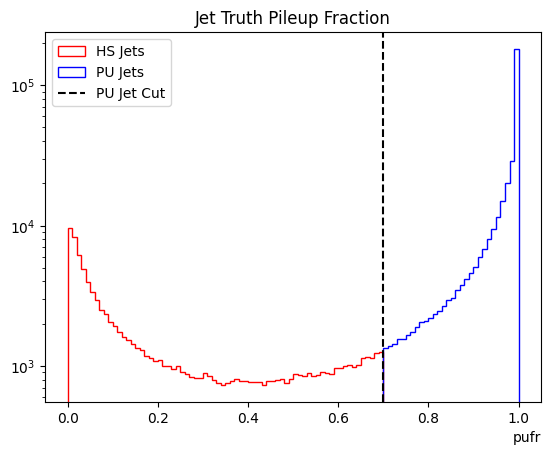
\includegraphics[width=0.3\textwidth]{PU_Jet_Cut}
\caption{An arbitrary cut on the continuous $PU_{fr}$ to recover binary labels.}
\end{figure}

\subsection{Classical JVT Architecture}\hfill

The Jet Vertex Tagger, JVT, was orignally proposed by ATLAS~\cite{ATLAS-CONF-2014-018}. The model uses $R_{pT}$ and corrJVF as input and constructs a likelihood between zero and one which represents the probability in which the jet originated from hard scatter. The JVT model is based on a k-Nearest Neighbor, kNN, algorithm which uses a Euclidean metric in the $R_{pT}$-corrJVF plane and is fit using k=100.

\begin{figure}[h!]
\centering
\begin{subfigure}{.3\textwidth}
  \centering
  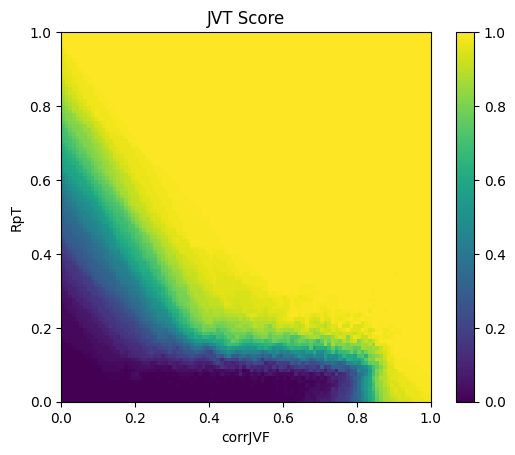
\includegraphics[width=0.9\linewidth]{JVT_2d}
  \caption{}
  \label{fig:sub1}
\end{subfigure}%
\begin{subfigure}{.3\textwidth}
  \centering
  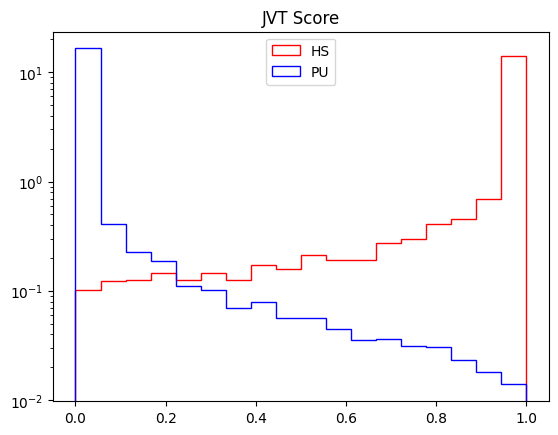
\includegraphics[width=1\linewidth]{JVT_1d}
  \caption{}
  \label{fig:sub2}
\end{subfigure}
\caption{Figure (a) shows JVT liklihood in the $R_{pT}$-corrJVF plane. Figure (b) shows the JVT liklihood for HS and PU jets.}
\label{fig:test}
\end{figure}

\subsection{AttnJVT Architecure}\hfill

To perform a fair benchmark, the orignal JVT model was recreated and performance was evaluated between the original model and the attention model on the same dataset. The input to the model is a unordered set of jets from an event. Each event has a variable number of jets, N, so the input tensor will be of shape $\mathbb{J} \in \mathbb{R}^{N,F}$ where F is the six input features described in section 2.1. The input jets are fed through an initializer, $\phi$, to transform them into the embedding space with dimension D:

\begin{equation}
\phi(\mathbb{J}) \rightarrow \mathbb{E} \in \mathbb{R}^{N,D} 
\end{equation}

The embedded jets are then passed through a multi-head attention layer to update their representations in the context of an entire event. First the embeddings $\mathbb{E}$ are passed through a multi-head attention layer using self attention to generate the context tensor $\mathbb{C}$:

\begin{equation}
\mathbb{C} = MHA(\mathbb{E},\mathbb{E},\mathbb{E})
\end{equation}

Then the context tensor, $\mathbb{C} \in \mathbb{R}^{N,D}$, is concatenated with the original embedding to update the original representation of each jet, $\mathbb{E} = \mathbb{E}+\mathbb{C}$. Lastly, the jet embedding is passed through a final classifier, $\Psi$, to perform binary classification:

\begin{equation}
\Psi(\mathbb{E}) \rightarrow \vec{y} \in \{0,1\}
\end{equation}

The model is trained using the Binary Cross Entropy loss function.

\begin{figure}[h!]
\centering
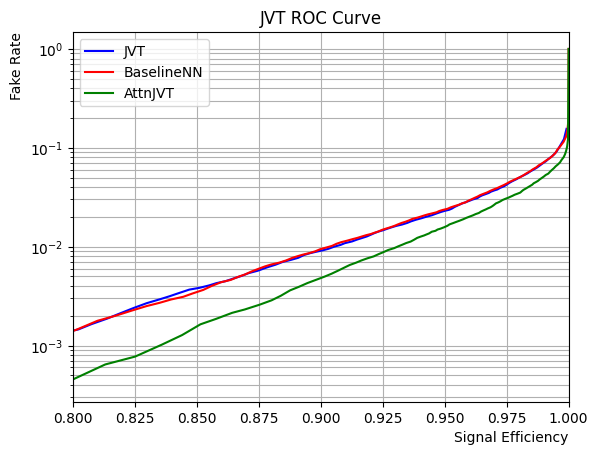
\includegraphics[width=0.5\textwidth]{AttnJVT}
\caption{Using a MHA layer, the jets have access to the context of the entire event which allows the model to capture correlations between HS jets. This effect reduces the fake rate of the model.}
\label{fig:test}
\end{figure}


\hfill\\
\section{Hogwild Attention}\hfill

This section describes how to predict the Efrac and Mfrac of a jet using a stack of Transformer Encoders using Multi-Head Attention layers in the context of an event using track features and jet features as input.

\subsection{Model Input}\hfill

The model takes an entire event as an input. An event can be described as three tensors: jet tensor, jet-track tensor, and all-track tensor. Jet tensor $\mathbb{J}\in \mathbb{R}^{N_{jets} \times F_{jets}}$ has shape N jets per event with F input features, $p_T, \eta, \phi, m$. Jet-Track tensor $\mathbb{T}_{jet}\in \mathbb{R}^{N_{jets} \times N_{trks} \times F_{trks}}$ has shape number of jets per event, number of tracks per jet, and number of features per track, $p_T, \eta, \phi, q, d_0, z_0$. Lastly, All-Track tensor $\mathbb{T}_{Event}\in \mathbb{R}^{\times N_{trks} \times F_{trks}}$ has shape number of tracks per event and features per track. Each of these tensors if first passed through a linear preprocessing layer to transform them into the embedding space.

\subsection{Encoders Architecture}\hfill

Four transformer encoder stacks are used to enrich each tensor -- $\mathbb{J},\mathbb{T}_{jet},\mathbb{T}_{jet}$ -- with context from the event. Each encoder follows the NormFormer [*] architecture by (... et al). NormFormers conist of LayerNorms, LN(), multi-head attention, MHA(), skip connections, + operator, feed-forward network, FFN, which consists of a linear layer and a GELU activation function. These layers are the components of each encoder block.

First, each jet is enriched with associated tracks. Since each jet only carries four features, $p_T, \eta, \phi, m$, tracks within a radius of $\Delta R = 0.4$ are used in the first encoder stack to achieve a rich representation of each jet.

\begin{align}
    \mathbb{T}_{context} &= \mathbb{T}_{jet} + LN(MHA(LN(\mathbb{T}_{jet}), LN(\mathbb{T}_{jet}), LN(\mathbb{T}_{jet}))) \\
    \mathbb{T}_{embed} &= \mathbb{T}_{context} + FFN (\mathbb{T}_{context}) \\
    \mathbb{T}_{aggregated} &= \sum_{dim=1} \mathbb{T}_{embed} \\ 
    \mathbb{J}_{enriched} &= FFN(\mathbb{J} \mathop{\oplus}_{dim=1} \mathbb{T}_{aggregated})
\end{align}
$\mathbb{T}_{jet}$, $\mathbb{T}_{context}$, and $\mathbb{T}_{embed}$ all have shape $N_{jet} \times N_{trk} \times E_{dim}$. Then the summation operator reduces the $N_{trk}$ dimension which will then match the dimension of $\mathbb{J}$ with shape $N_{jet} \times E_{dim}$. The jet and aggregated track tensors are concatenated along the embedding dimension, and the FFN has input $N_{jet} \times 2\cdot E_{dim}$ and outputs $\mathbb{J}$ of shape $N_{jet} \times E_{dim}$. This encoder block can be interpreted physically as learning to enrich the jet in the context of associated particles. For example, if there is are particles that resemble b-hadron decay, this encoder block might enrich this jet as a b-jet in the latent space.

Second, $\mathbb{T}_{event}$ with shape $N_{trk} \times E_{dim}$ are enriched using an encoder block using self-attention:
\begin{align}
    \mathbb{T}_{context} &= \mathbb{T}_{event} + LN(MHA(LN(\mathbb{T}_{event}), LN(\mathbb{T}_{event}), LN(\mathbb{T}_{event}))) \\
    \mathbb{T}_{embed} &= \mathbb{T}_{context} + FFN (\mathbb{T}_{context}) \\
\end{align}
The purpose of this encoder is to update all tracks in the context of the event and initialize them for cross attention with jets.

Third, cross attention between $\mathbb{J}_{enriched}$ and $\mathbb{T}_{embed}$ is performed to update the jets in the context of all tracks of the event.

\begin{align}
    \mathbb{J}_{context} &= \mathbb{J}_{enriched} + LN(MHA(LN(\mathbb{J}_{enriched}), LN(\mathbb{T}_{event}), LN(\mathbb{T}_{event}))) \\
    \mathbb{J}_{embed} &= \mathbb{J}_{context} + FFN (\mathbb{J}_{context}) \\
\end{align}

This encoder allows tracks to update the jet embedding in the context of an event. For example, if we consier $t \rightarrow Wb \rightarrow l\nu b$, this encoder allows the high energy lepton, l, to update the context of the b-jet.

Fourth and finally, $\mathbb{J}_{embed}$ with shape $N_{jet} \times E_{dim}$ is enriched using a encoder block using self attention:

\begin{align}
    \mathbb{J}_{context} &= \mathbb{J}_{embed} + LN(MHA(LN(\mathbb{J}_{embed}), LN(\mathbb{J}_{embed}), LN(\mathbb{J}_{embed}))) \\
    \mathbb{J}_{embed} &= \mathbb{J}_{context} + FFN (\mathbb{J}_{context}) \\
\end{align}

This encoder is performed last because at this stage the jets have achieved a rich representation after passing through the previous encoders. This last encoder allows jets to update their representation in the context of an event. This encoder can be interpreted physically as allowing jets to update representations according to conservation of momentum or other properties that might be shared between jets.

Lastly, the embedded jet vectors are passed through a final classification layer to predict the continuous pileup fraction label.

\subsection{Results}\hfill

The model was constructed using a stack of 3x jet associated-track encoders, 3x all track encoders, 3x jet all track encoders, and finally 3x jet encoders. In total the model has 4.1M parameters and took about 1 hour to converge on an NVIDIA 3090 using a sample size of 10k $t\bar{t}$ events with around 500k jets and 10M charged tracks greater than 400 MeV.

\begin{figure}[h!]
\centering
\begin{subfigure}{.25\textwidth}
  \centering
  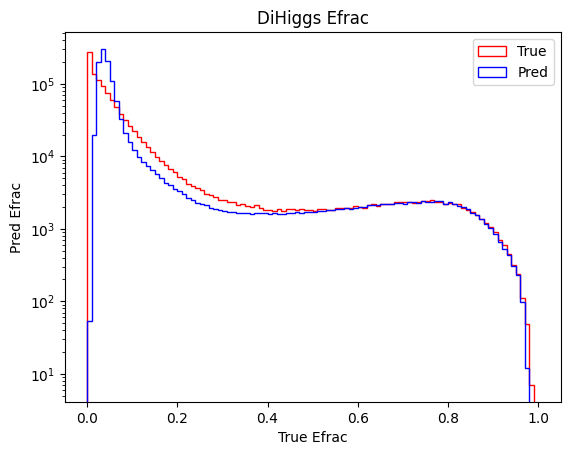
\includegraphics[width=1\linewidth]{diHiggs_Efrac_1d.png}
  \caption{}
  \label{fig:sub1}
\end{subfigure}%
\begin{subfigure}{.25\textwidth}
  \centering
  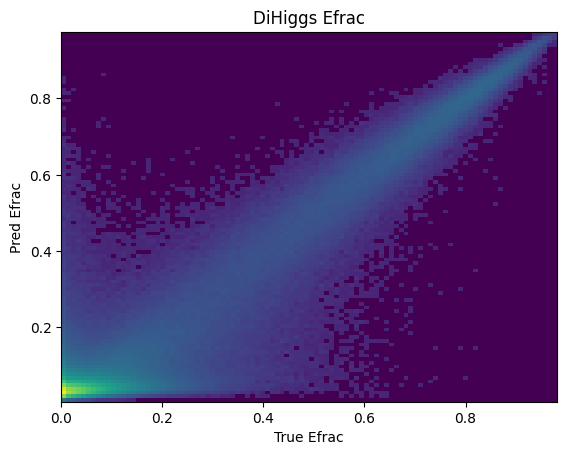
\includegraphics[width=1\linewidth]{diHiggs_Efrac_2d.png}
  \caption{}
  \label{fig:sub2}
\end{subfigure}
\begin{subfigure}{.25\textwidth}
  \centering
  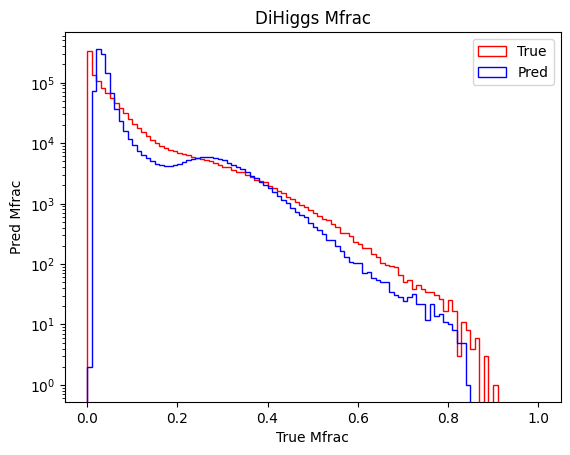
\includegraphics[width=1\linewidth]{diHiggs_Mfrac_1d.png}
  \caption{}
  \label{fig:sub1}
\end{subfigure}%
\begin{subfigure}{.25\textwidth}
  \centering
  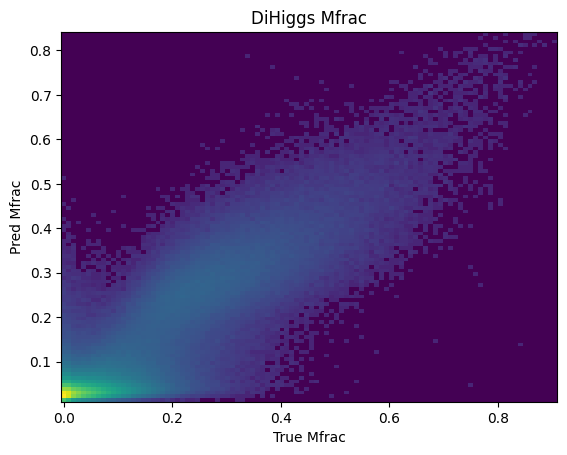
\includegraphics[width=1\linewidth]{diHiggs_Mfrac_2d.png}
  \caption{}
  \label{fig:sub2}
\end{subfigure}
\caption{The predicted Mass fraction of jets. Figure (a) 1-D Histogram. Figure (b) 2-D Historgram.}
\label{fig:test}
\end{figure}

\begin{figure}[h!]
\centering
\begin{subfigure}{.45\textwidth}
  \centering
  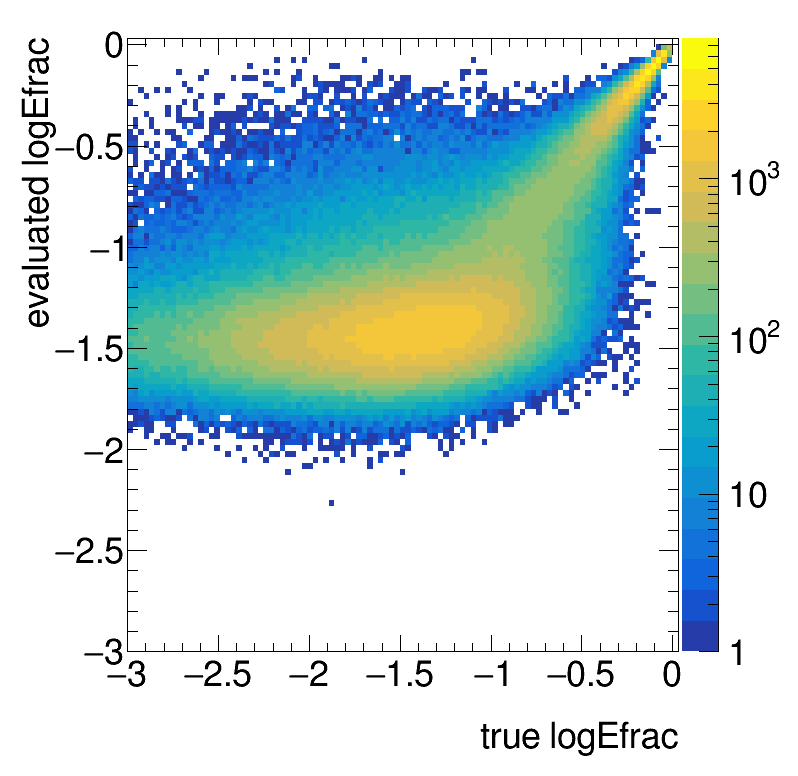
\includegraphics[width=1\linewidth]{logEfrac_eval_vs_true_HH_mu60_20k.png}
  \caption{}
  \label{fig:sub1}
\end{subfigure}%
\begin{subfigure}{.45\textwidth}
  \centering
  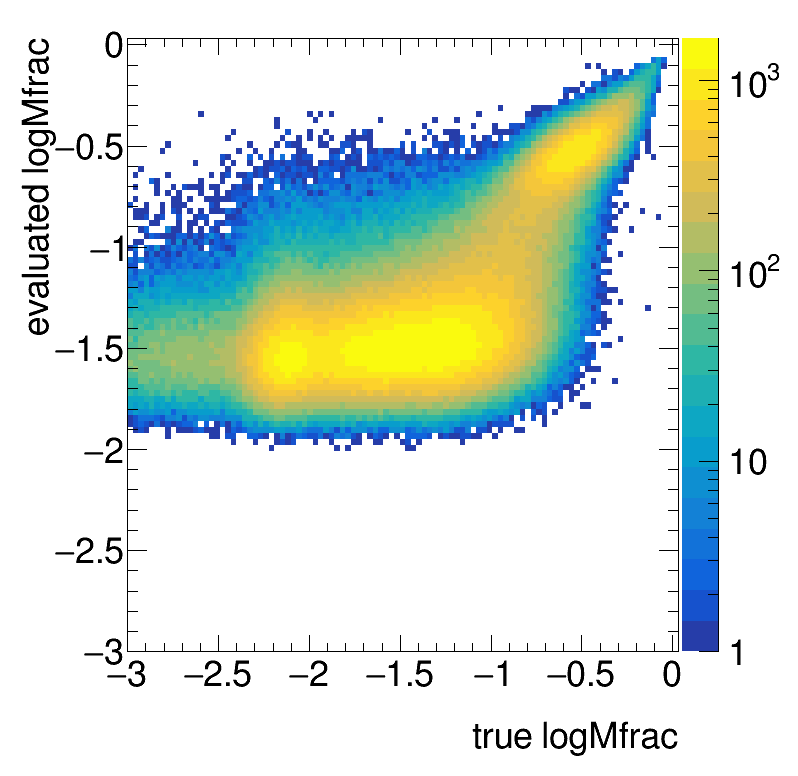
\includegraphics[width=1\linewidth]{logMfrac_eval_vs_true_HH_mu60_20k.png}
  \caption{}
  \label{fig:sub2}
\end{subfigure}
\caption{The predicted fractions vs the true fraction on a log scale. Figure (a) Efrac. Figure (b) Mfrac.}
\label{fig:test}
\end{figure}

\begin{center}
\begin{tabular}{||c c ||} 
 \hline
 Metric & Value  \\ [0.5ex] 
 \hline\hline
 Train Loss & 0.0016  \\ 
 \hline
 Val Loss & 0.0018 \\
 \hline
 Test Loss & 0.0022\\
 \hline
 Test MAE & 0.017 \\
 \hline
 Test RMSE & 0.046 \\ [1ex] 
 \hline
\end{tabular}
\end{center}

The model is trained using mean squared error loss. After converging, the train loss reaches around 0.00164, validation loss of about 0.0018, and train loss of 0.0022. The mean absolute error, MAE, of about 0.017, and the root mean squared error, RMSE, of about 0.046.



\section{Analysis}\hfill

In order to determine if the model is able to provide useful insight into a practical physics analysis, we attempt to reconstruct the Higgs mass from DiHiggs decaying to 4b events with a non-resonant 4b background. The non-resonant 4b sample has a 60GeV pTB filter applied at generation level to ensure the kinematics of each sample are indistinguishable. Therefore, the only difference between these samples is the the resonant mass peak that appears in the DiHiggs sample and the flat background from the non-resonant 4b sample.

Using the results of the Efrac and Mfrac model, we are able to apply jet corrections and see 

\begin{figure}[h!]
    \centering
    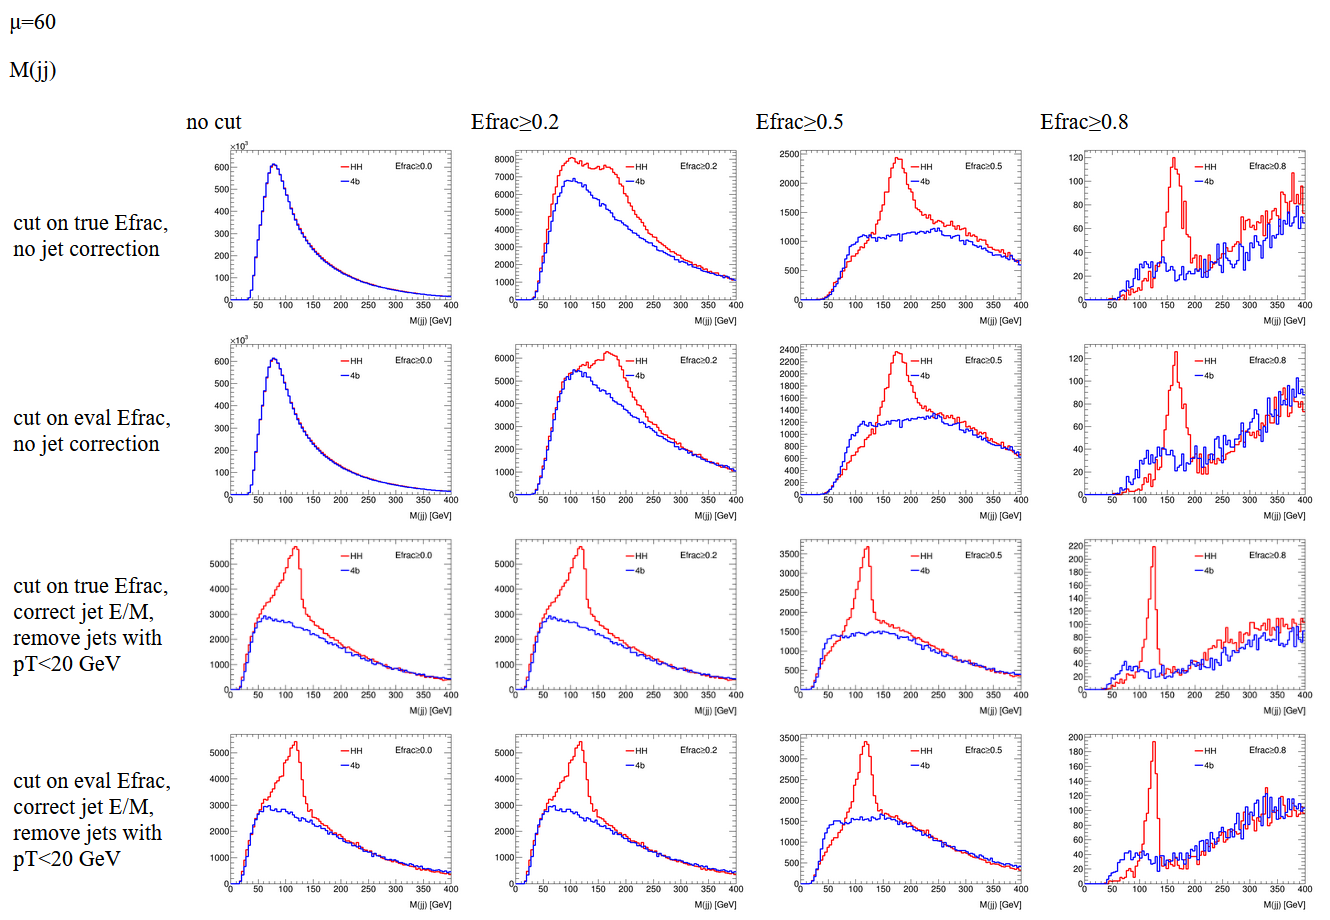
\includegraphics[width=1\linewidth]{tmp.png}
    \caption{Physics Analysis Results}
\end{figure}


\section{Conclusion}\hfill

In conclusion, we presented the following contributions.
\begin{enumerate}
    \item We proposed a first-of-its-kind pileup prediction modeled as a regression problem.
    \item We proposed a cross-attention based neural network architecture that utilizes jets and tracks information for pileup fraction detection.
    \item We showed with extensive analysis that the proposed method outperforms the baseline approaches.
    \item We also showed that the predictions from the proposed approach also assist with physics processes.
\end{enumerate}


\chapter{Pileup Studies Updated}
\section{Appendix A}
Here is A.

\section{Appendix B}
Here is B.


\chapter{More Appendix}
\section{Appendix A}
Here is A.

\section{Appendix B}
Here is B.


\end{document}
